\subsection{\hl{Camera Software Test}}
\label{app:camera_software_test}
\subsubsection*{Introduction}

Much of the camera functionality is verified by analysis and compared with software provided by ZWO (ASICAP). For example the library written in the IRISC software produces an image of the correct format with the correct file size and the correct header content (more header content can still be added in necessary). To analyze noise differences two tests are made:

\begin{enumerate}
    \item The IRISC software is compared with the ASICAP software provided by ZWO.
    \item Connecting the camera via USB 2 and USB 3 is compared using the IRISC software.
\end{enumerate}

\subsubsection*{Method \& Setup}

The telescope is set up on vibration dampening legs facing a building wall roughly 50 meters away.

For test 1, the camera is connected to a laptop over USB 3. Next the IRISC software in run which captures ten images. That is followed by capturing ten images using ASICAP.  For test 2, the camera is connected to a RPi 4B through USB 3. The IRISC software then captures ten images. The camera is then disconnected and reconnected through a USB 2 port and another ten images are captured after a few seconds to let any vibrations caused by moving the table to die down. Two comparisons are made in each test:

\begin{enumerate}
    \item The sets of images from each software are averaged pixel wise and a difference between the means is calculated. The mean and standard deviation of the distribution of the pixels in this diff image is analyzed to find if any noise is added consistently. 

    \item The differences between the images in each set is investigated.  This is done by subtracting the mean pixel wise from each image and analyzing the standard deviation of the resulting distribution.
\end{enumerate}

\subsubsection*{Result}

\paragraph{Test 1, Comparison 1 (T1C1)}\,\\

The result from the first comparison follows a normal distribution, $ N( -0.393, 21.4^2 ) $.

\paragraph{Test 1, Comparison 2 (T1C2)}\,\\

The images from the IRISC software follow the normal distribution $ N( 0, 43.2^2 ) $.
The images from ASICAP follow the normal distribution $ N( 0, 43.4^2 ) $.
The total time required to capture the images was 6 and 32 seconds respectively for the two softwares.

\paragraph{Test 2, Comparison 1 (T2C1)}\,\\

The distribution in T2C1 can be estimated with a heavily skewed normal distribution, $ N( 349, 82.2^2 ) $ with a skewness of 90.2. Figure \ref{usb_comp} shows this distribution.

\begin{figure}[H]
    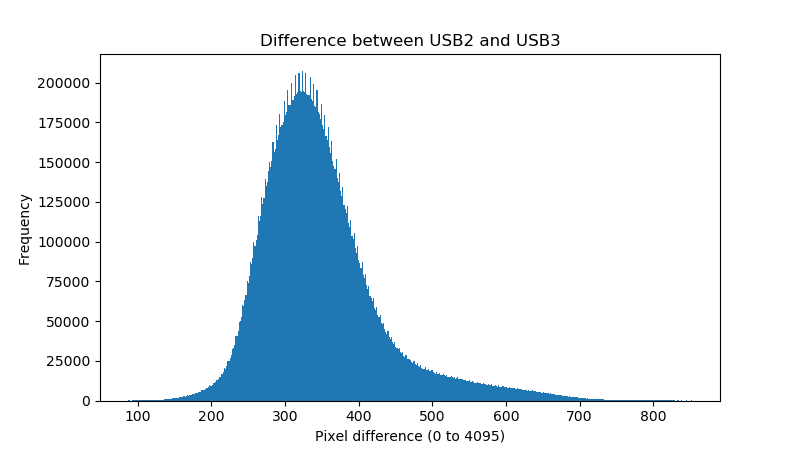
\includegraphics[width=\textwidth]{appendix/img/test-results/camera_software_test.png}
    \caption{The distribution of the pixel wise difference USB 2 - USB 3 for image capturing.}
    \label{usb_comp}
\end{figure}

\paragraph{Test 2, Compatison 2 (T2C2)}\,\\

The images taken over USB 2 and 3 follow the distributions $ N( 0, 59.6^2 ) $ and $ N( 0, 41.1^2 ) $ respectively. The distributions have a slight positive skew of 0.141 and 0.025 respectively. The total time required to capture the images was 30 and 10 seconds respectively for the two interfaces.

\vspace{-.3cm}
\subsubsection*{Discussion}

The mean difference between the images captured using IRISC software and using ASICAP of -0.393 is within margin of error. Considering that the sensor has a 12 bit ADC resulting in 4096 possible values, a standard deviation of 41 corresponds to $1\%$ of the maximum pixel value. Since there is a small time difference between each image capture and since the sensor isn't perfect, there will be some random noise added. Therefore the standard deviation of T1C1 can be assumed to be independent of the software used. Since the standard deviations of T1C2 are almost equal, it can be concluded that the IRISC software doesn't introduce any noise when compared to ASICAP.\\

\vspace{-.1cm}
The result from T2C1 and the almost 50\% higher standard deviation in T2C2 shows that there is a lot of noise added when the camera is operated over USB 2. This is due to the camera not having an onboard memory buffer as mentioned in section 6.8 in the camera manual (\href{https://astronomy-imaging-camera.com/manuals/ASI183\%20Manual\%20EN.pdf}{link, page 12}). This means that the data is read directly from the sensor. Therefore, the slower the data is read the more noise will be added. Because of this we will either need to upgrade to the Pro version of the camera or upgrade to a RPi 4B to avoid noise since the currently used RPi 3B+ does not have USB 3 capabilities. Upgrading to the Pro camera version is not recommended due to costs but it is noteworthy that there is probably noise added without memory buffer even when using USB 3.